%\documentclass[manuscript]{biometrika}
\documentclass[lineno]{biometrika}

\usepackage{mathtools}  % amsmath with extensions
\usepackage{amsfonts}  % (otherwise \mathbb does nothing)

%% Please use the following statements for
%% managing the text and math fonts for your papers:
\usepackage{times}
%\usepackage[cmbold]{mathtime}
\usepackage{bm}
\usepackage{natbib}
\usepackage{optidef}

\usepackage[noend,linesnumbered]{algorithm2e}

\makeatletter
\renewcommand{\algocf@captiontext}[2]{#1\algocf@typo. \AlCapFnt{}#2} % text of caption
\renewcommand{\AlTitleFnt}[1]{#1\unskip}% default definition
\def\@algocf@capt@plain{top}
\renewcommand{\algocf@makecaption}[2]{%
  \addtolength{\hsize}{\algomargin}%
  \sbox\@tempboxa{\algocf@captiontext{#1}{#2}}%
  \ifdim\wd\@tempboxa >\hsize%     % if caption is longer than a line
    \hskip .5\algomargin%
    \parbox[t]{\hsize}{\algocf@captiontext{#1}{#2}}% then caption is not centered
  \else%
    \global\@minipagefalse%
    \hbox to\hsize{\box\@tempboxa}% else caption is centered
  \fi%
  \addtolength{\hsize}{-\algomargin}%
}
\makeatother

%%% User-defined macros should be placed here, but keep them to a minimum.
\def\Bka{{\it Biometrika}}
\def\AIC{\textsc{aic}}
\def\T{{ \mathrm{\scriptscriptstyle T} }}
\def\v{{\varepsilon}}

\addtolength\topmargin{35pt}
\DeclareMathOperator{\Thetabb}{\mathcal{C}}

\begin{document}

%% Here are the title, author names and addresses
\title{Mixture Proportion Estimation via Kernel Embedding of Distributions for Identifying Target Observations}

\author{Stewart Kerr, Guanhua Chen, Menggang Yu}
\affil{Department of Biostatistics and Medical Informatics \\ University of Wisconsin-Madison}

\maketitle

\begin{abstract}
Mixture proportion estimation (MPE) via kernel embedding was explored theoretically and with simulation studies. Preliminary results indicate that MPE via kernel embedding is viable and yields high accuracy estimates. Two different methods of implementing the algorithm were tested and one was found to yield higher accuracy estimates in all cases. A preliminary study of extending the method to identify target observations in the mixture was performed and results were promising. Future work includes further exploration of the algorithm, testing the algorithm with real data, and applying the enhanced algorithm to clinical/EHR domain data.
\end{abstract}

\section{Introduction}
Mixture proportion estimation (MPE) is the problem of estimating the weight of a component distribution in a mixture given samples from the mixture (source) and component (target). Solving this problem is an important step in “weakly supervised” learning tasks in which one has access to only positively labelled data or there is noise in the labels in the training set. Specifically, we are interested in MPE to assess the similarity between two different populations of hospital patients. For example, we develop models that create a "priority score" for each elligible patient. The priority score combines the predicted positive effect of our particular intervention ("benefit score") and the predicted outcome of the patient without any intervention ("risk score") into one measure that helps prioritize which patients should receive the intervention. Our model is developed using historical electronic health record ("EHR") and medical claims data for a subset of eligible patients in the University of Wisconsin Health System. While our model was trained on a specific population, we wish to extend this model to create priority scores for patients in other health systems. Specifically, we have a partnership with the University of Iowa Health Care System to deploy our priority scoring methods to their patient population. However, despite geographical proximity to Wisconsin, there is no gaurantee that eligible patients in the Iowa system will be similar to Wisconsin patients used to develop the priority scoring model. Thus, the first step is to generate some measure of similarity between the two health systems, in the form of the proportion of eligible Iowa patients which are similar to Wisconsin patients, and then to determine which of these eligible Iowa patients most closely resemble the Wisconsin patient population. 

Among several methods proposed to solve MPE problems, we adapt methods proposed by \citet{Ramaswamy:2016} via kernel embedding of distributions. This approach utilizes an efficient algorithm for MPE along with guaranteed convergence to estimate the true proportion under certain less restrictive conditions than previous methods. Using this method, we can obtain a similarity estimate, $\hat{\kappa}$, of the proportion of the source population that matches the target population. However, we wish to extend this mixture proportion estimatation method to identify the $\hat{\kappa}$ proportion of observations from the source population which most closely match the target. Successful identification of these observations will allow us to target our priority score models only to eligible patients that are most similar to the patients used to train the model.  To identify these observations, we propose using SVM classification methods to estimate a separating hyperplane to discriminate the source and target populations (figure 1). Specifically, we will build an SVM classifier using the same kernel used for MPE estimation above. SVM is a desirable approach because distance from each observation to the separating hyperplane provides a direct measure of how similar an observation from the target population is to samples in the source population. 

\begin{figure}[h]
\begin{center}
% The arguments in the next line are {height}{optional width}{used only by OUP for typesetting}[filename, in directory art]
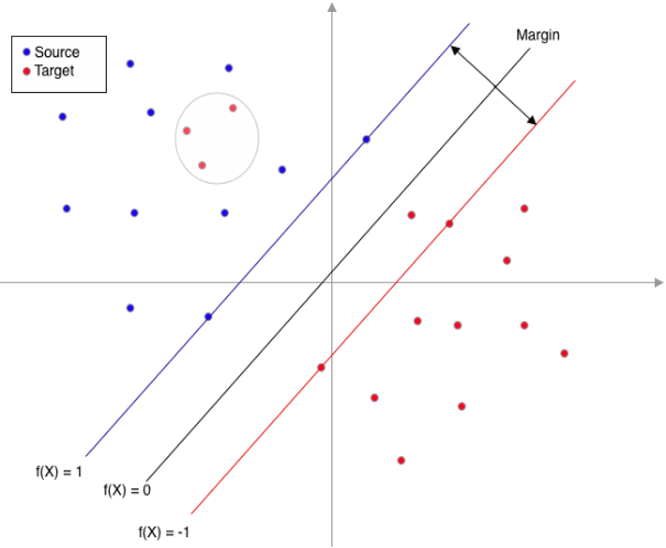
\includegraphics[width=0.65\linewidth, height=0.6\linewidth]{art/svm.png}
% note that files may not be rotated
\caption{SVM classification for mixture of target and source populations}
\label{fig1}
\end{center}
\end{figure}


For the purposes of this report, existing code published by \citet{Ramaswamy:2016} is explored with the intent of gaining a deeper understanding of MPE methods for subsequent research tasks outlined above.  Specifically, simulations of different mixture and component samples are performed at varying mixture levels, sample sizes, and dimensionality to assess the algorithm's accuracy, runtime, and robustness.

\section{Background}
The mixture proportion estimation problem can be formalized as follows. Let $G, H$ be distributions over a compact metric space $\chi$. Let $\kappa^* \in [0,1)$ and let $F$ be a distribution that is given by a mixture of $G$ and $H$: 

\begin{center}
$F = (1-\kappa^* )G + \kappa^* H$
\end{center}

We can rearrange to find G:

\begin{center}
$G = (\lambda^*)F + (1-\lambda^*)H, $ 
\end{center}

\begin{center}
$\lambda^* = \frac{1}{1-\kappa^*}$ 
\end{center} 

$F$ represents the \textbf{source} population, $H$ represents the \textbf{target} population, and $G$ represents the subset of the source population which is \textit{not} from the target. Thus, $F$ corresponds to the Iowa patient population, $H$ corresponds to the Wisconsin patient population, and $G$ corresponds to the subset of the Iowa population which is not similar to the Wisconsin population. Given two samples $\{x_1,x_2,...,x_n\}$ drawn i.i.d from $F$ and $\{x_{n+1},...x_{n+m}\}$ drawn i.i.d from $H$, the task at hand is to estimate $\kappa^*$ - the proportion of the mixture or source population which is generated from the target population distribution \citep{Ramaswamy:2016}. \newline

To estimate $\kappa^*$ we embed the distributions in a reproducing kernel Hilbert space (RKHS) with a unique positive semi-definite kernel matrix $ K : \chi \times \chi \to \mathbb{R} $ \citep{Manton:2015}. Intuitively, we can view these kernels as a mapping of a vector from some subspace to a higher dimensional space, called the embedding space, in which an action can be performed on the vector before mapping back to a point in the subspace. Because the operation returns an element of the original subspace, we call it \textit{reproducing}. An example of the reproducing property of the kernel $K$ is that an arbitary vector $v$ can be returned by taking the inner product wit respect to the columns $k_i$ of $K$: 

\begin{center}
$v = (\langle v,k_1\rangle, ... ,\langle v,k_n\rangle)$. 
\end{center}  

Now, let $\phi : \chi \to \mathcal{H}$ represent the kernel mapping $x \in \chi \to K(x,x^*)$. This mapping can be thought of as the inner product of $x$ with some other element $x^* \in \chi$ in a higher dimensional $\chi \times \chi$ space \citep{Wahba:2002}. Now, for any distribution $P$ over $\chi$ define $\phi(P) = E_{X\sim P}\phi(X)$ as the expected value of the kernel mapping of distribution $P$. Let $\Delta_{n+m} \subseteq \mathbb{R}^{n+m}$ be the $(n+m-1)$-dimensional probability simplex defined as $ \Delta_{n+m} = \{\mathbf{p} \in [0,1]^{n+m} : \sum_i p_i = 1\}$. The probability simplex can be thought of as a tetrahedron in $(n+m-1)$ dimensional space which encompasses valid probabilities over the observed data. Let $C, C_s$ be defined as:

\begin{center}
$C = \{w \in \mathcal{H} : w = \phi (P)\}$ 
\end{center}
\begin{center}
$C_S = \{w \in \mathcal{H}: w = \sum\limits_{i=1}^{n+m} \alpha_i \phi (x_i) $ for some $\alpha \in \Delta_{n+m}\}$.
\end{center}

Note that for the mixture of $F = (1-\kappa^* )G + \kappa^* H$, in which we observe both $F$ and $H$, the task is to compute $\phi(G)$. We expect $G$ to have cardinality $n/\lambda^*$, but since $G$ is unknown we cannot compute $\phi(G)$ directly and must instead use the RKHS distance.

Define the "$C$-distance" function $d: [0,\infty) \to [0,\infty)$ as:

\begin{center}
$d(\lambda) = \underset{w\in C}{\textrm{inf}} || \lambda \phi(F) + (1-\lambda)\phi(H) - w ||_{\mathcal{H}}$
\end{center}

This function reconstructs the kernel embedding of G, $\phi (G)$ from $F$ and $H$. The emperical version of this function, based on the observed data, is defined as:

\begin{center}
$\hat{d}(\lambda) = \underset{w\in C_S}{\textrm{inf}} || \lambda \phi(\hat{F}) + (1-\lambda)\phi(\hat{H}) - w ||_{\mathcal{H}}$
\end{center}

Which can be formulated as the quadratic optimization problem:

\begin{center}
$(\hat{d}(\lambda))^2 = \underset{v\in \Delta_{n+m}}{\textrm{inf}} (\mathbf{u}_{\lambda} - \mathbf{v})^T K(\mathbf{u}_{\lambda} - \mathbf{v})$
\end{center}

Where K is the kernel matrix defined above as $K_{i,j} = k(x_i,x_j)$ and $\mathbf{u}_{\lambda} \in \mathbb{R}^{n+m} : \mathbf{u}_{\lambda}^T = \frac{\lambda}{n}([\mathbf{1}_n^T,\mathbf{0}_m^T]) + \frac{(1-\lambda)}{m}([\mathbf{0}_n^T,\mathbf{1}_m^T])$. Intuitively, the kernel matrix calculates the similarity between two observations and the task is to find the vector of probabilities $v$ which minimizes the distance between the mixture and target population. The algorithm for solving this problem is detailed next.

\section{Methods}

One approach to estimating $\hat{d}(\lambda)$ is through the use of a gradient thresholding estimator. For some $v \in [0,\infty)$ the gradient thresholding estimator is defined as:

\begin{center}
$\hat{\lambda}^G_v = \textrm{inf}\{\lambda : \exists g \in \delta \hat{d}(\lambda), g\ge v\}$,
\end{center}

where $\delta \hat{d}(\lambda)$ is the sub-differential of $\hat{d}(.)$ at $\lambda$, which is non-decreasing as $\hat{d}(.)$  is a convex function. Thus, using the gradient thresholding estimator is a viable strategy to estimate $\lambda^*$.

Under certain assumptions on separability conditions, namely that $G$ cannot be expressed as a non-trivial mixture of the target population $H$ and some other distribution, then the gradient thresholding estimator will converge to $\lambda^*$ efficiently using binary search. The algorithm below is used to compute $\hat{\lambda}^G_v = \hat{\lambda^*}$.

\subsection{Algorithm}

\begin{algorithm}[!h]
\caption{Kernel mean based gradient thresholder}
\begin{tabbing}
\qquad \enspace \textbf{Input:} $x_1,x_2,...,x_n$ drawn from mixture F and $x_{n+1},...,x_{n+m}$ drawn from component $H$\\
\qquad \enspace \textbf{Parameters:} $k : \chi \times \chi \to [0,\infty),  v \in [0,\infty) $\\
\qquad  \enspace \textbf{Output:} $\hat{\lambda}^G_v$\\
\qquad \enspace \textbf{Constants:} $\epsilon, \lambda_{\textrm{UB}}, \lambda_{\textrm{left}} = 1, \lambda_{\textrm{right}} = \lambda_{\textrm{UB}}, K_{i,j} = k(x_i,x_j)$ for $1 \le i, j \le n + m$ \\
\qquad \enspace \textbf{while} $\lambda_{\textrm{right}} - \lambda_{\textrm{left}} \ge \epsilon:$ \\
\qquad \qquad \enspace $\lambda_{\textrm{curr}} = \frac{\lambda_{\textrm{right}} + \lambda_{\textrm{left}}}{2} $ \\
\qquad \qquad \enspace $\lambda_1 = \lambda_{\textrm{curr}}- \epsilon / 4 $ \\
\qquad \qquad \enspace $\mathbf{u_1}  = \frac{\lambda_1}{n} ([\mathbf{1}_n^T, \mathbf{0}_m^T]) + \frac{1-\lambda_1}{m} ([\mathbf{0}_n^T, \mathbf{1}_m^T])$ \\
\qquad \qquad \enspace $d_1 = \hat{d}(\lambda_1)^2 = \underset{\mathbf{v}\in\Delta_{n+m}}{\textrm{min}} (\mathbf{u}_1 - \mathbf{v})^T K (\mathbf{u}_1 - \mathbf{v}) $ \\
\qquad \qquad \enspace $\lambda_2 = \lambda_{\textrm{curr}} + \epsilon / 4 $ \\
\qquad \qquad \enspace $\mathbf{u_2}  = \frac{\lambda_2}{n} ([\mathbf{1}_n^T, \mathbf{0}_m^T]) + \frac{1-\lambda_2}{m} ([\mathbf{0}_n^T, \mathbf{1}_m^T])$ \\
\qquad \qquad \enspace $d_2 = \hat{d}(\lambda_2)^2 = \underset{\mathbf{v}\in\Delta_{n+m}}{\textrm{min}} (\mathbf{u}_2 - \mathbf{v})^T K (\mathbf{u}_2 - \mathbf{v}) $ \\
\qquad \qquad \enspace $s = \frac{\sqrt{d_2} - \sqrt{d_1}}{\lambda_2 - \lambda_1} $ \\
\qquad \qquad \enspace \textbf{if} $s > v$: \\
\qquad \qquad \qquad \enspace $\lambda_{\textrm{right}} = \lambda_{\textrm{curr}} $ \\
\qquad \qquad \enspace \textbf{else}: \\
\qquad \qquad \qquad \enspace $\lambda_{\textrm{left}} = \lambda_{\textrm{curr}} $ \\
\qquad \enspace \textbf{return} $\lambda_{\textrm{curr}}$
\end{tabbing}
\end{algorithm}

The algorithm works by establishing upper $(\lambda_{\textrm{right}})$ and lower $(\lambda_{\textrm{left}})$ bounds on the estimated $\lambda$ which are adjusted based on the computed slope at the current estimate $(\lambda_{\textrm{curr}})$. The value of $\hat{d}(\lambda)$ can be computed using any convex programming solver. 

There are two parameters of interest for this algorithm: the kernel embedding $k$ and the threshold $v$ for adjusting the uppe/lower bounds. Any kernel can be chosen, but the kernel which maximizes the RKHS distance between the mixture and component distributions is preferred. The RKHS distance is equal to the slope of $\hat{d}$ at $\infty$, thus choosing the kernel which maximizes RKHS will yield larger gradients for optimization which leads to faster convergence. There are two strategies to select the gradient threshold $v$. The first is to set $v = 1/\sqrt{\textrm{min}(m,n)}$. The second is to choose $v$ as a convex combination of the initial slope of $\hat{d}$ at $\lambda = 1$ and the final slope at $\lambda = \infty$. These two strategies are denoted KM1 and KM2 respectively. This algorithm was implemented in Python and the focus of the rest of this report is in examining the performance of this algorithm on simulated data.

\subsection{Simulations}

In order to explore the effectiveness of this MPE approach, simulation studies were performed with the intent to gain additional understanding before applying the algorithm to real data. Two datasets were generated, one a mixture of the target population and some other distribution and the other consisting only of the target population. With these two simulated datasets, there are a number of aspects to consider, including sample size, number/distribution of variables, and true proportion of the target population in the mixture. As an initial test, a $500$ observation, $100$ variable mixture population was generated with $200$ observations from the normal distribution with mean $10$ and standard deviation $1$ and the remaining $300$ observations being generated from the standard normal distribution $(\kappa = 0.4)$. The proportion estimation produced by the algorithm was highly accurate for both strategies KM1 and KM2, thus the algorithm was deemed highly effective in this simple case (table 1). \newline

\begin{table}[h]
\def~{\hphantom{0}}
\tbl{}{%
\begin{tabular}{lcccc}
 \\
& KM1 & KM2 \\
$\kappa^*$ & 0.40 & 0.40 \\
$\hat{\kappa^*}$  & 0.3912 & 0.4012 \\
Absolute Error & 0.0084 & 0.0012 \\
\end{tabular}}
\label{tablelabel}
\begin{tabnote}
\center{Results of MPE Algorithm in simple case with $n = 500$}
\end{tabnote}
\end{table}

Next, the sample size, number/distribution of variables, and true proportion was varied while keeping other inputs constant. Specifically, inputs were set to mirror the above test case - the total number of observations was fixed to $500$, $\kappa^*$ was fixed to $0.4$, the number of covariates was fixed to $100$, and the mean of the component distribution was fixed to $10$.  The results are shown in figure 2.

\begin{figure}[t]
% The arguments in the next line are {height}{optional width}{used only by OUP for typesetting}[filename, in directory art]
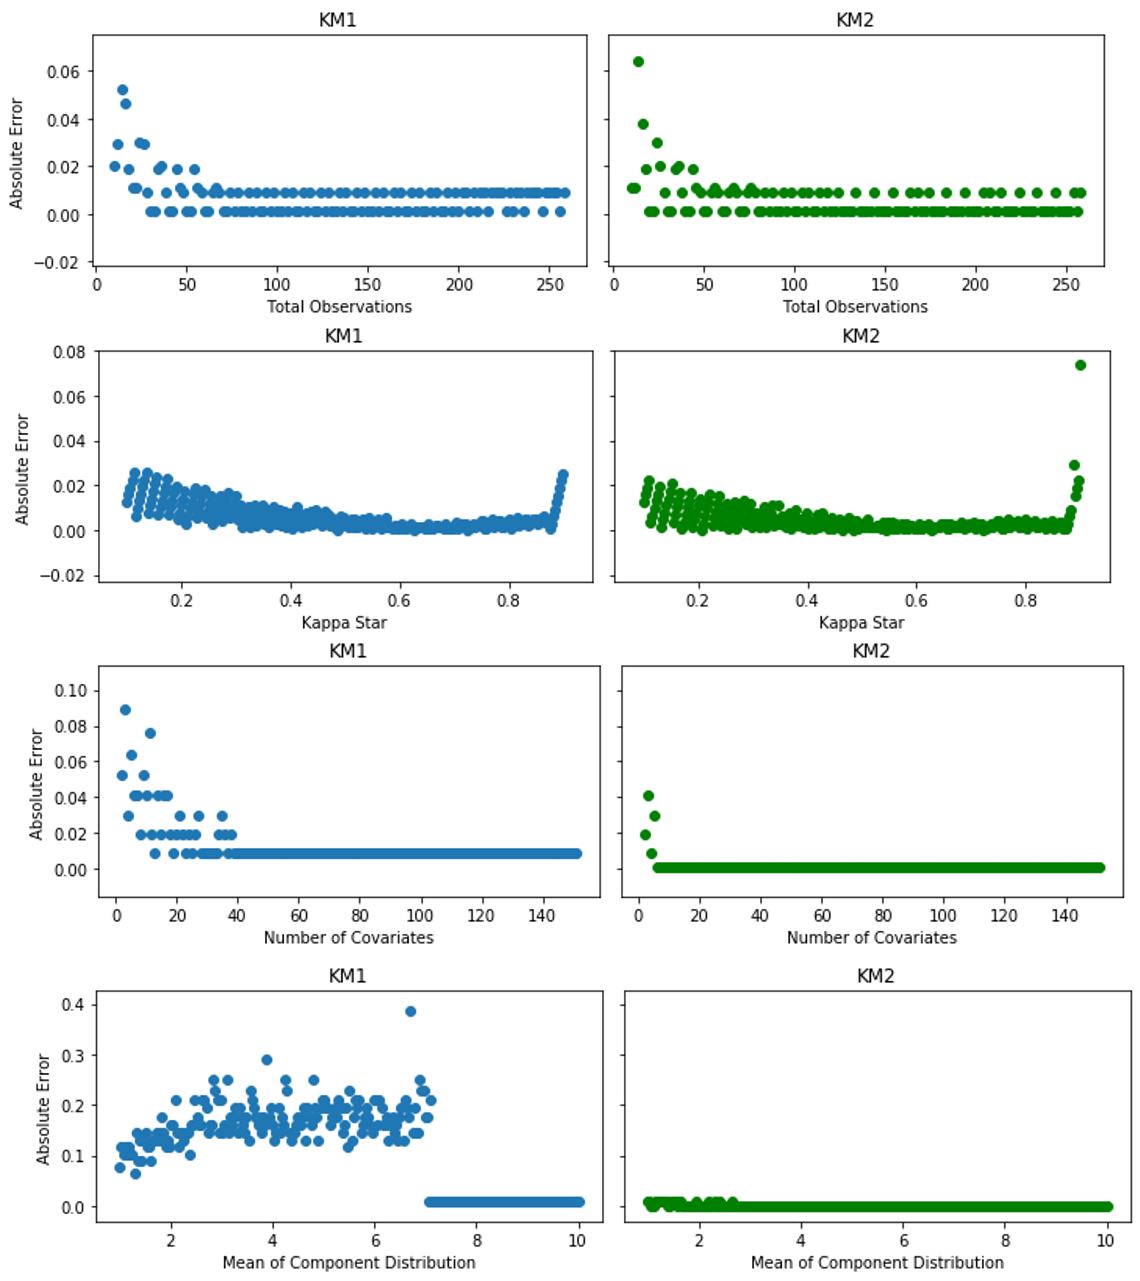
\includegraphics[width=1\linewidth, height=1\linewidth]{art/sim_results.png}
% note that files may not be rotated
\caption{Simulation results from varying inputs to the MPE algorithm}
\label{fig2}
\end{figure} 

\section{Results}
Although the simulated data used to produce the results in figure 2 are very simple, a number of important considerations are immediately evident. It appears that, at least for the simple case, KM2 outperforms KM1 in almost every scenario. Thus, for future studies, when the true proportion is unknown, results from the KM2 method will be treated as more accurate and used as the proportion estimate. Now, we consider each of the varied inputs separately.

\subsection{Total Observations}
Here the number of total observations in the mixture (which includes observations from both the target population and the population we are not interested in) was varied from $10$ to around $250$ while keeping all other inputs equal (see above) and absolute error was measured. Overall, absolute error was never higher than $0.06$ and, as expected, the algorithms yield more accurate predictions as we increase the sample size. KM2 outperforms KM1 beginning at about 100 total observations and KM2 appears to improve accuracy with more observations while KM1 does not. It's interesting that error oscillates between approximately $0.01$ and close to $0$ for both gradient thresholding strategies - I would like to further explore this pattern to determine if it's a systematic error. Our Wisconsin and Iowa data includes thousands of patients, thus the algorithm will likely work well given our sample size.

\subsection{True Mixture Proportion}
The point of the MPE is to estimate the true mixture proportion, this it's highly imperative that we understand how the algorithm behaves at different mixture proportion values. Overall, absolute error is never higher than 0.08 for either gradient thresholding algorithms and was below 0.04 for the vast majority of tests. One would expect that the algorithm would perform worse at low and high mixture proportions, which is reflected in our simulation study. Interestingly, the algorithm appears to be most accurate around $\kappa^* = 0.65$ but errors within the range $\kappa^* = [0.4, 0.8]$ are all low. Both KM1 and KM2 appear to have similar performance as $\kappa^*$ is varied. My conclusions from these results are that if the MPE algorithm predicts a $\kappa^*$ within the $[0.4,0.8]$ range, then the prediction is likely more trustworthy than a prediction outside of that range. 

\subsection{Number of Covariates}
The covariates for both the target population and the population not of interest in the mixture were generated from the normal distribution with standard deviation $1$. For this study, the target population had mean $10$ while the population not of interest had mean $1$. This is a very simplistic case and does not accurately reflect the reality of our data, which includes many binary variables, but it's a useful starting point to explore the effect of covariates. For this study, KM2 vastly outperformed KM1 at lower number of covariates but the two methods are relatively equal as the size of the data increases. For KM2, we really only need a few variables for the algorithm to predict the true mixture proportion with high accuracy. For our purposes, we perform a significant reducation on the dimensionality of the data before generating priority scores, thus, KM2 will be the preferred approach.

\subsection{Distance between Distributions}
As mentioned above, the covariates for both populations were generated from the normal distribution. The algorithm works by computing RKHS distance, thus one would expect the algorithm to perform better when the underlying distributions are further apart. Interestingly, KM2 actually performs very well even if the distributions of the covariates are very similar. On the other hand, KM1 is highly inaccurate if the covariates are similar in distribution. This study is too simple for any real dataset, but the key takeaway for me is that the KM2 gradient thresholding approach is again preferable to KM1.

\subsection{Runtime}
As both time and computing power are a limited resource, runtime is an important aspect to consider when selecting an algorithm. For our task, we have thousands of patients with hundreds of covariates, thus, it's important to examine how the algorithm scales with increasing data. For this study, the algorithm's runtime was measured as the number of total observations in the mixture was varied from $500$ to $5000$ in increments of $100$ while keeping everything else constant (figure 3). 

\begin{figure}[h]
% The arguments in the next line are {height}{optional width}{used only by OUP for typesetting}[filename, in directory art]
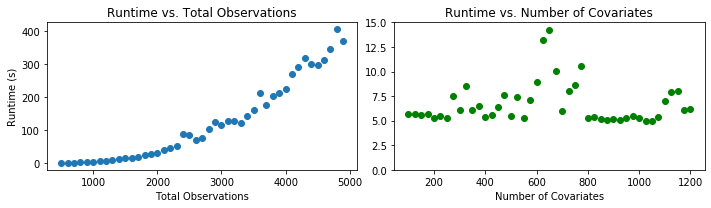
\includegraphics[width=1\linewidth]{art/runtime_results.png}
% note that files may not be rotated
\caption{Runtime results for varying input data sizes}
\label{fig3}
\end{figure} 

From the simulation studies, it appears that the runtime grows weakly exponentially with the total number of observations while number of covariates has little to no effect on runtime. Note that due to the nature of these simulation studies, both results are affected by random fluctuations in the data. The algorithm never took more than about 400 seconds to complete which is sufficiently quick for the size of our data (which includes only thousands of patients and hundreds of covariates). However, thousands of observations is still relatively small, thus for larger, more complex data problems this algorithm may not be computationally feasible.

\section{Identification of Target Observations}
From the simulation results, its evident that the algorithm can accurately predict the true mixture proportion for a large data mixture particularly if the KM2 method is used. In this section, we extend estimation of the mixture proportion towards selecting the specific observations from the mixture which are most similar to the target population. Within the MPE algorithm, the distances that are calculated $(d_1, d_2)$ can be intuitively thought of as the probability that a particular observation comes from $G$, the nuisance population in the mixture, rather than $H$, the target population. Thus, once we have calculated $\kappa^*$, the estimated mixture proportion, we can return to the distance vector calculated during the final iteration of the algorithm and select the $\kappa^*$-proportion of observations in the mixture which have the \textbf{lowest} probability of being generated by G. These are the observations in the mixture which are most similar to the target population.

The MPE code published by Ramaswamy was slightly modified so that the algorithm returns both $\kappa^*$ as well as the optimization solution, including the distance vector, from the final iteration of the algorithm. Then, a test using simulated data was conducted in which a known mixture population was constructed - that is, observations generated from the target population in the mixture were labelled as such. After generating the mixture, the algorithm was run to estimate both the mixture proportion and distance vector using the KM2 method. From the distance vector, the $\kappa^*$ proportion of observations with the highest likelihood of being generated from the component distribution were selected and compared to the known labels. This process was simulated 100 times under conditions nearly identical to the simulation studies above and the results are provided in table 2.

\begin{table}[h]
\def~{\hphantom{0}}
\tbl{}{%
\begin{tabular}{lcccc}
 \\
$\kappa^*$ & 0.40 \\
Total Observations in Mixture & $500$ \\
Target Observations in Mixture & $200$ \\
Average $\hat{\kappa^*}$  & 0.401 \\
Average Misclassification Rate & 0.0252 \\
\end{tabular}}
\label{tablelabel}
\begin{tabnote}
\center{Average misclassification rate of observations generated from the target distribution.}
\end{tabnote}
\end{table}

The results from this simple, preliminary experiment are promising. The average misclassification rate among the 100 simulations was around 0.025, indicating that this could be a viable approach to identify the target population within the mixture. Further studies with increasingly complicated simulated data would be useful to better understand the efficacy of this method.
\newpage

\section{Conclusion}

The Kernel Embedding approach to MPE proposed by \citet{Ramaswamy:2016} was detailed and explored in order to gain a deeper understanding of the method and insight into its performance. Using simple simulated data, the algorithm was shown to perform well with errors generally around $0.01$. Furthermore, insight into characteristics of the input mixture was gathered via simulation studies and it was found that the KM2 approach to gradient thresholding is preferred. Thus, this algorithm is a good candidate for MPE to identify the proportion of Iowa patients that are similar to Wisconsin patients.  As the algorithm calculates and stores RKHS distance, we can extend the algorithm to identify which observations are most similar (that is, have smallest distance to known target observations). This extension of the algorithm was explored and preliminary results appear promising. Next steps for this research include further simulation studies to examine the performance of the algorithm under increasingly difficult conditions, further studies on extracting the observations in the mixture which are most similar to the target population, and eventually using the algorithm on real data - possibly the Wisconsin/Iowa patient data.

\vspace*{-10pt}

%\bibliographystyle{biometrika}
%\bibliography{paper-ref}


\begin{thebibliography}{7}
\expandafter\ifx\csname natexlab\endcsname\relax\def\natexlab#1{#1}\fi

\bibitem[{Ramaswamy(2016)}]{Ramaswamy:2016}
\textsc{Ramaswamy, G. H., Scott, C. \& Tewari, A.} (2016).
\newblock Mixture Proportion Estimation via Kernel Embedding of Distributions
\newblock \textit{arXiv}: 1603.02501v2

\bibitem[{Manton(2015)}]{Manton:2015}
\textsc{Manton, J. H., \& Amblard, P.} (2015).
\newblock \textit{{A Primer on Reproducing Kernel Hilbert Spaces}}.
\newblock Foundations and Trends in Signal Processing
\newblock \textit{arXiv}: 1408.0952v2 

\bibitem[{Wahba(2002)}]{Wahba:2002}
\textsc{Wahba, G.} (2002).
\newblock \textit{{Soft and hard classification by reproducing kernel Hilbert space methods}}.
\newblock \textit{PNAS} \textbf{99}, 16524--16530.
\newblock \textit{arXiv}: 10.1073/pnas.242574899

\bibitem[{Vandenberghe(2012)}]{Vandenberghe:2012}
\textsc{Andersen, M.S., Dahl, J. \& Vandenberghe, L.} (2012).
\newblock CVXOPT: A Python package for convex optimization, version 1.1.5

\end{thebibliography}

\end{document}
